
%% bare_conf.tex
%% V1.4b
%% 2015/08/26
%% by Michael Shell
%% See:
%% http://www.michaelshell.org/
%% for current contact information.
%%
%% This is a skeleton file demonstrating the use of IEEEtran.cls
%% (requires IEEEtran.cls version 1.8b or later) with an IEEE
%% conference paper.
%%
%% Support sites:
%% http://www.michaelshell.org/tex/ieeetran/
%% http://www.ctan.org/pkg/ieeetran
%% and
%% http://www.ieee.org/

%%*************************************************************************
%% Legal Notice:
%% This code is offered as-is without any warranty either expressed or
%% implied; without even the implied warranty of MERCHANTABILITY or
%% FITNESS FOR A PARTICULAR PURPOSE! 
%% User assumes all risk.
%% In no event shall the IEEE or any contributor to this code be liable for
%% any damages or losses, including, but not limited to, incidental,
%% consequential, or any other damages, resulting from the use or misuse
%% of any information contained here.
%%
%% All comments are the opinions of their respective authors and are not
%% necessarily endorsed by the IEEE.
%%
%% This work is distributed under the LaTeX Project Public License (LPPL)
%% ( http://www.latex-project.org/ ) version 1.3, and may be freely used,
%% distributed and modified. A copy of the LPPL, version 1.3, is included
%% in the base LaTeX documentation of all distributions of LaTeX released
%% 2003/12/01 or later.
%% Retain all contribution notices and credits.
%% ** Modified files should be clearly indicated as such, including  **
%% ** renaming them and changing author support contact information. **
%%*************************************************************************


% *** Authors should verify (and, if needed, correct) their LaTeX system  ***
% *** with the testflow diagnostic prior to trusting their LaTeX platform ***
% *** with production work. The IEEE's font choices and paper sizes can   ***
% *** trigger bugs that do not appear when using other class files.       ***                          ***
% The testflow support page is at:
% http://www.michaelshell.org/tex/testflow/



\documentclass[conference]{IEEEtran}
% Some Computer Society conferences also require the compsoc mode option,
% but others use the standard conference format.
%
% If IEEEtran.cls has not been installed into the LaTeX system files,
% manually specify the path to it like:
% \documentclass[conference]{../sty/IEEEtran}





% Some very useful LaTeX packages include:
% (uncomment the ones you want to load)


% *** MISC UTILITY PACKAGES ***
%
%\usepackage{ifpdf}
% Heiko Oberdiek's ifpdf.sty is very useful if you need conditional
% compilation based on whether the output is pdf or dvi.
% usage:
% \ifpdf
%   % pdf code
% \else
%   % dvi code
% \fi
% The latest version of ifpdf.sty can be obtained from:
% http://www.ctan.org/pkg/ifpdf
% Also, note that IEEEtran.cls V1.7 and later provides a builtin
% \ifCLASSINFOpdf conditional that works the same way.
% When switching from latex to pdflatex and vice-versa, the compiler may
% have to be run twice to clear warning/error messages.

\usepackage{cite}
\usepackage{amsmath,amssymb,amsfonts}
\usepackage{algorithmic}
\usepackage{algorithm}
\usepackage{graphicx}
\usepackage{gensymb}
\usepackage{textcomp}
%	\usepackage[strings]{underscore}
\usepackage{tikz}
\usetikzlibrary{calc,patterns,angles,quotes,shapes,arrows, chains}


% *** CITATION PACKAGES ***
%
%\usepackage{cite}
% cite.sty was written by Donald Arseneau
% V1.6 and later of IEEEtran pre-defines the format of the cite.sty package
% \cite{} output to follow that of the IEEE. Loading the cite package will
% result in citation numbers being automatically sorted and properly
% "compressed/ranged". e.g., [1], [9], [2], [7], [5], [6] without using
% cite.sty will become [1], [2], [5]--[7], [9] using cite.sty. cite.sty's
% \cite will automatically add leading space, if needed. Use cite.sty's
% noadjust option (cite.sty V3.8 and later) if you want to turn this off
% such as if a citation ever needs to be enclosed in parenthesis.
% cite.sty is already installed on most LaTeX systems. Be sure and use
% version 5.0 (2009-03-20) and later if using hyperref.sty.
% The latest version can be obtained at:
% http://www.ctan.org/pkg/cite
% The documentation is contained in the cite.sty file itself.






% *** GRAPHICS RELATED PACKAGES ***
%
\ifCLASSINFOpdf
% \usepackage[pdftex]{graphicx}
% declare the path(s) where your graphic files are
% \graphicspath{{../pdf/}{../jpeg/}}
% and their extensions so you won't have to specify these with
% every instance of \includegraphics
% \DeclareGraphicsExtensions{.pdf,.jpeg,.png}
\else
% or other class option (dvipsone, dvipdf, if not using dvips). graphicx
% will default to the driver specified in the system graphics.cfg if no
% driver is specified.
% \usepackage[dvips]{graphicx}
% declare the path(s) where your graphic files are
% \graphicspath{{../eps/}}
% and their extensions so you won't have to specify these with
% every instance of \includegraphics
% \DeclareGraphicsExtensions{.eps}
\fi
% graphicx was written by David Carlisle and Sebastian Rahtz. It is
% required if you want graphics, photos, etc. graphicx.sty is already
% installed on most LaTeX systems. The latest version and documentation
% can be obtained at: 
% http://www.ctan.org/pkg/graphicx
% Another good source of documentation is "Using Imported Graphics in
% LaTeX2e" by Keith Reckdahl which can be found at:
% http://www.ctan.org/pkg/epslatex
%
% latex, and pdflatex in dvi mode, support graphics in encapsulated
% postscript (.eps) format. pdflatex in pdf mode supports graphics
% in .pdf, .jpeg, .png and .mps (metapost) formats. Users should ensure
% that all non-photo figures use a vector format (.eps, .pdf, .mps) and
% not a bitmapped formats (.jpeg, .png). The IEEE frowns on bitmapped formats
% which can result in "jaggedy"/blurry rendering of lines and letters as
% well as large increases in file sizes.
%
% You can find documentation about the pdfTeX application at:
% http://www.tug.org/applications/pdftex





% *** MATH PACKAGES ***
%
%\usepackage{amsmath}
% A popular package from the American Mathematical Society that provides
% many useful and powerful commands for dealing with mathematics.
%
% Note that the amsmath package sets \interdisplaylinepenalty to 10000
% thus preventing page breaks from occurring within multiline equations. Use:
%\interdisplaylinepenalty=2500
% after loading amsmath to restore such page breaks as IEEEtran.cls normally
% does. amsmath.sty is already installed on most LaTeX systems. The latest
% version and documentation can be obtained at:
% http://www.ctan.org/pkg/amsmath





% *** SPECIALIZED LIST PACKAGES ***
%
%\usepackage{algorithmic}
% algorithmic.sty was written by Peter Williams and Rogerio Brito.
% This package provides an algorithmic environment fo describing algorithms.
% You can use the algorithmic environment in-text or within a figure
% environment to provide for a floating algorithm. Do NOT use the algorithm
% floating environment provided by algorithm.sty (by the same authors) or
% algorithm2e.sty (by Christophe Fiorio) as the IEEE does not use dedicated
% algorithm float types and packages that provide these will not provide
% correct IEEE style captions. The latest version and documentation of
% algorithmic.sty can be obtained at:
% http://www.ctan.org/pkg/algorithms
% Also of interest may be the (relatively newer and more customizable)
% algorithmicx.sty package by Szasz Janos:
% http://www.ctan.org/pkg/algorithmicx




% *** ALIGNMENT PACKAGES ***
%
%\usepackage{array}
% Frank Mittelbach's and David Carlisle's array.sty patches and improves
% the standard LaTeX2e array and tabular environments to provide better
% appearance and additional user controls. As the default LaTeX2e table
% generation code is lacking to the point of almost being broken with
% respect to the quality of the end results, all users are strongly
% advised to use an enhanced (at the very least that provided by array.sty)
% set of table tools. array.sty is already installed on most systems. The
% latest version and documentation can be obtained at:
% http://www.ctan.org/pkg/array


% IEEEtran contains the IEEEeqnarray family of commands that can be used to
% generate multiline equations as well as matrices, tables, etc., of high
% quality.




% *** SUBFIGURE PACKAGES ***
%\ifCLASSOPTIONcompsoc
%  \usepackage[caption=false,font=normalsize,labelfont=sf,textfont=sf]{subfig}
%\else
%  \usepackage[caption=false,font=footnotesize]{subfig}
%\fi
% subfig.sty, written by Steven Douglas Cochran, is the modern replacement
% for subfigure.sty, the latter of which is no longer maintained and is
% incompatible with some LaTeX packages including fixltx2e. However,
% subfig.sty requires and automatically loads Axel Sommerfeldt's caption.sty
% which will override IEEEtran.cls' handling of captions and this will result
% in non-IEEE style figure/table captions. To prevent this problem, be sure
% and invoke subfig.sty's "caption=false" package option (available since
% subfig.sty version 1.3, 2005/06/28) as this is will preserve IEEEtran.cls
% handling of captions.
% Note that the Computer Society format requires a larger sans serif font
% than the serif footnote size font used in traditional IEEE formatting
% and thus the need to invoke different subfig.sty package options depending
% on whether compsoc mode has been enabled.
%
% The latest version and documentation of subfig.sty can be obtained at:
% http://www.ctan.org/pkg/subfig




% *** FLOAT PACKAGES ***
%
%\usepackage{fixltx2e}
% fixltx2e, the successor to the earlier fix2col.sty, was written by
% Frank Mittelbach and David Carlisle. This package corrects a few problems
% in the LaTeX2e kernel, the most notable of which is that in current
% LaTeX2e releases, the ordering of single and double column floats is not
% guaranteed to be preserved. Thus, an unpatched LaTeX2e can allow a
% single column figure to be placed prior to an earlier double column
% figure.
% Be aware that LaTeX2e kernels dated 2015 and later have fixltx2e.sty's
% corrections already built into the system in which case a warning will
% be issued if an attempt is made to load fixltx2e.sty as it is no longer
% needed.
% The latest version and documentation can be found at:
% http://www.ctan.org/pkg/fixltx2e


%\usepackage{stfloats}
% stfloats.sty was written by Sigitas Tolusis. This package gives LaTeX2e
% the ability to do double column floats at the bottom of the page as well
% as the top. (e.g., "\begin{figure*}[!b]" is not normally possible in
% LaTeX2e). It also provides a command:
%\fnbelowfloat
% to enable the placement of footnotes below bottom floats (the standard
% LaTeX2e kernel puts them above bottom floats). This is an invasive package
% which rewrites many portions of the LaTeX2e float routines. It may not work
% with other packages that modify the LaTeX2e float routines. The latest
% version and documentation can be obtained at:
% http://www.ctan.org/pkg/stfloats
% Do not use the stfloats baselinefloat ability as the IEEE does not allow
% \baselineskip to stretch. Authors submitting work to the IEEE should note
% that the IEEE rarely uses double column equations and that authors should try
% to avoid such use. Do not be tempted to use the cuted.sty or midfloat.sty
% packages (also by Sigitas Tolusis) as the IEEE does not format its papers in
% such ways.
% Do not attempt to use stfloats with fixltx2e as they are incompatible.
% Instead, use Morten Hogholm'a dblfloatfix which combines the features
% of both fixltx2e and stfloats:
%
% \usepackage{dblfloatfix}
% The latest version can be found at:
% http://www.ctan.org/pkg/dblfloatfix




% *** PDF, URL AND HYPERLINK PACKAGES ***
%
%\usepackage{url}
% url.sty was written by Donald Arseneau. It provides better support for
% handling and breaking URLs. url.sty is already installed on most LaTeX
% systems. The latest version and documentation can be obtained at:
% http://www.ctan.org/pkg/url
% Basically, \url{my_url_here}.




% *** Do not adjust lengths that control margins, column widths, etc. ***
% *** Do not use packages that alter fonts (such as pslatex).         ***
% There should be no need to do such things with IEEEtran.cls V1.6 and later.
% (Unless specifically asked to do so by the journal or conference you plan
% to submit to, of course. )


% correct bad hyphenation here
\hyphenation{op-tical net-works semi-conduc-tor}


\begin{document}
	%
	% paper title
	% Titles are generally capitalized except for words such as a, an, and, as,
	% at, but, by, for, in, nor, of, on, or, the, to and up, which are usually
	% not capitalized unless they are the first or last word of the title.
	% Linebreaks \\ can be used within to get better formatting as desired.
	% Do not put math or special symbols in the title.
	%\title{Bare Demo of IEEEtran.cls\\ for IEEE Conferences}
%	\tableofcontents
	\title{ROCO504\\ Catch-bot}
	
	% author names and affiliations
	% use a multiple column layout for up to three different
	% affiliations
	\author{\IEEEauthorblockN{Tom Queen}
		\IEEEauthorblockA{School of Computing,\\ Electronics and Mathematics\\
			Plymouth University\\
			Plymouth, Devon PL4 8AA \\
			Email: xxxx}
		\and
		\IEEEauthorblockN{Daniel Gregory-Turner}
		\IEEEauthorblockA{School of Computing,\\ Electronics and Mathematics\\
			Plymouth University\\
			Plymouth, Devon PL4 8AA \\
			Email: xxxx}
		\and
		\IEEEauthorblockN{Demetrius Zaibo}
		\IEEEauthorblockA{School of Computing,\\ Electronics and Mathematics\\
			Plymouth University\\
			Plymouth, Devon PL4 8AA \\
			Email: xxxx}}
	
	% conference papers do not typically use \thanks and this command
	% is locked out in conference mode. If really needed, such as for
	% the acknowledgment of grants, issue a \IEEEoverridecommandlockouts
	% after \documentclass
	
	% for over three affiliations, or if they all won't fit within the width
	% of the page, use this alternative format:
	% 
	%\author{\IEEEauthorblockN{Michael Shell\IEEEauthorrefmark{1},
	%Homer Simpson\IEEEauthorrefmark{2},
	%James Kirk\IEEEauthorrefmark{3}, 
	%Montgomery Scott\IEEEauthorrefmark{3} and
	%Eldon Tyrell\IEEEauthorrefmark{4}}
	%\IEEEauthorblockA{\IEEEauthorrefmark{1}School of Electrical and Computer Engineering\\
	%Georgia Institute of Technology,
	%Atlanta, Georgia 30332--0250\\ Email: see http://www.michaelshell.org/contact.html}
	%\IEEEauthorblockA{\IEEEauthorrefmark{2}Twentieth Century Fox, Springfield, USA\\
	%Email: homer@thesimpsons.com}
	%\IEEEauthorblockA{\IEEEauthorrefmark{3}Starfleet Academy, San Francisco, California 96678-2391\\
	%Telephone: (800) 555--1212, Fax: (888) 555--1212}
	%\IEEEauthorblockA{\IEEEauthorrefmark{4}Tyrell Inc., 123 Replicant Street, Los Angeles, California 90210--4321}}
	
	
	
	
	% use for special paper notices
	%\IEEEspecialpapernotice{(Invited Paper)}
	
	
	
	
	% make the title area
	\maketitle
	
	% As a general rule, do not put math, special symbols or citations
	% in the abstract
	\begin{abstract}
This article discusses the development and construction of a Translational Planar 4-cable Cable-Direct-Driven Robot (CDDR), using soft robotics practices, and its applications in catching and throwing. The CDDR is tested for performance and reliability.
	\end{abstract}
	
	% no keywords
	
	
	
	
	% For peer review papers, you can put extra information on the cover
	% page as needed:
	% \ifCLASSOPTIONpeerreview
	% \begin{center} \bfseries EDICS Category: 3-BBND \end{center}
	% \fi
	%
	% For peerreview papers, this IEEEtran command inserts a page break and
	% creates the second title. It will be ignored for other modes.
	\IEEEpeerreviewmaketitle
	
	
	
	\section{Introduction}
	% no \IEEEPARstart
This article discusses the development and construction of a Translational Planar 4-cable Cable-Direct-Driven Robot (CDDR), using soft robotics practices, and its applications in catching and throwing. The CDDR is tested for performance and reliability.

Section \ref{research} of this document discusses the background research, linking to the main design challenges faced when constructing a catching robot. \ref{prototypes} details the various attempted solutions and their resultant outcomes. System capabilities are experimentally analysed in \ref{experiments}, followed by an overall summary in \ref{overall}.



\hfill January 4, 2018


\section{Design Process}
\subsection{Problem}
\subsubsection{Inverse Kinematics}\label{initial_kinematics}
Initially, it was thought that the commands to each motor could be generated by looking directly at the returned X and Y coordinates of the tracked objects. To move the gripper upwards, the top two motors should rotate clockwise and the bottom two anticlockwise. To move the gripper to the left, the two left motors should rotate clockwise and the right two anticlockwise. This led to the following kinematic solution:
\begin{equation}
\begin{aligned}
&M1 = Y - X \\
&M2 = Y + X\\
&M3 = -Y -X\\
&M4 = -Y + X\\
\end{aligned}
\end{equation}
For high torque motors, elastic cords and a closed loop between the tracked object and the gripper, this approximation may have been functional. However, it would not have been accurate, slack cords would be common and it would unnecessarily load the motors. When using stepper motors with low-current drivers, this solution caused the steppers to skip if the gripper was directed more than a few centimetres from the centre of the working area. 
This led to a re-evaluation of the kinematic solution as can be seen in section \ref{kinematic_solution_1}.

\subsubsection{Force storage} \label{force_problem}
For a robot to throw an object kinetic energy needs to be added to the system. To impart more force to the object than the motors can instantaneously provide a method of storing the force will have to be implemented.
\subsubsection{Hardware Requirements}
In order for a gripper to track a target, a low latency high FPS camera and fast motors will be needed. Section \ref{motorSpeedRequired} describes motor speed requirements and \ref{camera} describes the camera which was selected for this task.

\subsection{Research}\label{research}
The problem of designing and implementing a catching robot is not new, and although a thorough analysis of design considerations for catching robots in general is out of the scope of this article a brief summary of related issues will be outlined. The interested reader should read~\cite{Sorg2003VisualTA} for a more detailed analysis.

\subsubsection{Body Design}
Body design determines the shape of the overall robot, setting many project constraints such as the available workspace, control complexity and physical capabilities of the robot. There are numerous possible designs such as robot arms, as used by ~\cite{6810147}, ~\cite{malzahn2014modeling} and ~\cite{5980073}, or frame-based robots, as used by ~\cite{6385963}, and ~\cite{forpheus}. Due to project time constraints, a simple 2-axis frame based 4-cable CDDR was designed as the main body.

\subsubsection{Cable-Direct-Driven Robots}
Cable-Direct-Driven Robots (or CDDRs) are a type of parallel manipulator wherein the end-effector link is supported in parallel by $n$ cables with $n$ tensioning motors ~\cite{CDDR:description}. CDDRs can be made lighter, stiffer, safer and more economical than traditional serial robots~\cite{WilliamsII2003} since their primary structure consists of lightweight, high load-bearing cables. More complex Cable-driven parallel robots can be designed to move in six Degrees of Freedom (DoF) in three-dimensional space, but these are beyond the scope of this article. 

\subsubsection{Gripper Design}
Gripper design refers to the end effector which grasps the thrown object and constrains the design in what objects can be caught and how said objects can be manipulated. Gripper designs can be distinguished between 2 pairs of classes, passive verses active and soft verses hard.
In the first pairing, passive grippers provide no means of control within the gripper, simplifying design and control considerations but limits future capabilities. Active grippers increase the design and control complexity by adding actuation to perform a wider variety of tasks.
Hard grippers are constructed out of rigid, inflexible, materials. These grippers are commonplace within industry where they work with known objects that are strong enough to not break under high stresses. Outside of the industrial setting, however, they are less applicable. This is where soft grippers which can deform and spread the gripper forces over a larger surface area find more usage.

\subsubsection{Camera Setups}
Camera setups typically provide a trade-off between system complexity and control complexity. More cameras, or ones with higher frame rates and resolutions, allow for better object tracking but come at the cost of additional processing and control requirements.
There are two common camera setups.
\begin{itemize}
	\item The simplest setup for control is the eye-in-hand approach, where a camera is mounted inside the gripper, providing a direct feedback loop so long as motion blur doesn’t become an issue.
	\item The most reliable setup for object tracking involves placing multiple cameras around the room in fixed, known locations. From this, the ball position and trajectory can be easily modelled in 3D space, but at the expense of a complex setup and a significantly higher processor demand.

\end{itemize}
\subsubsection{Object Tracking}
Object tracking consumes the majority of processor resources in such projects. Accuracy, false positives and false negatives determine the reliability of a system. Cameras, and hence computer vision, provide numerous methods of feature detection. A small sample of such techniques include:
\begin{itemize}
	\item \textit{Colour thresholding}, whereby a colour range of interest is selected and a binary image is produced. Position is estimated using the centre of mass, or via structural analysis.
	\item \textit{Structural analysis} looks at the edges and corners in a given image in an attempt to detect predefined shapes.
	\item \textit{Statistical transformations} convert an image, or set of images, into fuzzy regions of interest. Blob detection, Farneback optical flow and convolution are examples of such methods.
	\item \textit{Depth maps}, generated from multiple images or through special hardware, provide a form of 3D representation of the environment, allowing other simpler algorithms to detect moving objects and the 3-dimensional direction of motion.
\end{itemize}
\subsubsection{Gripper-Object Coordination}
is the main control algorithm used in the catching process and defines the efficacy and efficiency of the system. It is usually broken down into numerous input and output controllers. Input controllers relate the sensory data to desired movements of the machine, and output controllers relate this desired motion into actuator commands.

Vision-based sensors can be used for visual servoing is, where an offset from the centre of the camera image directly translates to a velocity vector. Other systems employ predictive feedback, which predict possible locations the object will intersect the robot and provides this as a target location for the gripper.

The system can convert an input which directly relates to a desired gripper position into actual movements. This involves the use of kinematics, where forward kinematics provides an internal representation of the current system state, and inverse kinematics provide the actuator positions to attain the desired system state. For more complex systems, other parameters including the centre of mass and force storage may need to be taken into account. 

\subsubsection{Object Grasping}
Object grasping refers to post-catch manipulation of the object. More manipulability often implies more complex gripper designs. For instance ~\cite{1249273} use a high speed 3-fingered robotic hand to perform a wide variety of tasks, however, this approach is over-engineered if all that is required of the robot is to catch, a task a standard household bin can perform with the right aim.
For the purposes of the project presented in this article the two tasks of interest are the catching and throwing of an object.

\subsubsection{Motors}\label{motorSpeedRequired}
Fast motors were needed for the gripper to move quickly enough to catch an object. Our motor speed requirements were based off an object thrown from $2.5m$ away. The object would be thrown at a velocity of $5m/s$ at an angle of $45\degree$. The time of flight would be $721ms$ and the maximum height of the object would be $0.637m$. Worst case, the gripper would have to travel from corner to corner across the centre of the frame, resulting in a minimum travel speed of $1.635m/s$. If a spool diameter of $10cm$ was used, the required motor speed is $5.2\ RPS$ or $312\ RPM$.

\subsection{Methodology}
Given the problem breakdown discovered in the research, it was decided to split development into three sections; the first focussing on the frame design and hardware; the second looking into gripper designs and the control system including visual feedback.

For each section, many conceptual designs would be explored and analysed. Afterwards, all ideas would be reviewed and the most achievable and functional designs selected. Some of the analysis involved creating prototypes as there was insufficient information to make a practical decision otherwise.

After implementing all of the selected solutions, each section was tested for functionality. On success, the sections were integrated together and the whole system tested. Design flaws at this stage either meant an integration fault, or that flaws in a subsection weren't readily obvious when tested in isolation, hence taking longer to remedy. Finally, the system was tested for full functionality and reliability.


\subsection{Prototypes}\label{prototypes}
Throughout the project a lot of time was spent attempting to get a setup which could physically meet the aims of the project. To this end several design iterations occurred.

\subsubsection{Motors}
Two motor setups were prototyped. The first was to use high torque ($300Ncm$) encoded DC motors (E192.24.125), with a maximum speed of 33rpm. As the required motor speed was 312RPM and the micro motor could only provide 33rpm, a 1:9.45 ratio gearbox was required. Given the high torque output from the motors this should have provided enough speed and torque to move the gripper. However, even after many gearbox design iterations design flaws kept occurring, ranging from gear slippage to material failure. By making the length of each gear inversely proportional to its accumulated speed multiplier, the stress felt by the input gear could be spread out over the rest of the gears. However, this would have more than doubled the size of our original gearbox, as such it was determined that an alternative approach may yield better results.

The second prototype involved the use of SST58D3820 stepper motors from an old ER1 robot by Evolution Robotics. These motors are specified to hold $7.3Kg.cm$, dropping to $6.5Kg.cm$ at a frequency of 1200 pulses per second (PPS). In full step mode the stepper shaft rotates $1.8\degree$ per step. This translates to: \begin{equation}
\begin{aligned}
\frac{a\cdot p}{s} = \frac{1.8\cdot 1200}{360} = 6 RPS
\end{aligned}
\end{equation}
\begin{equation}
\begin{aligned}
\frac{\pi\cdot d\cdot a\cdot p}{s} = \frac{\pi \cdot 10 \cdot 1.8 \cdot 1200}{360} = 188.49 cm/s\\ 
%6\cdot\pi\cdot 10 = 188.49cm/s
\end{aligned}
\end{equation} Where $a$ is the step angle, $p$ is pulses per second, $d$ is the spool diameter ($10cm$) and $s$ is the desired speed in RPM. After a small amount of reverse engineering the motors were tested with their original motor driver which, unfortunately, did not appear to provide enough current to meet the motors torque limit; because of this the TB6600 motor driver was used instead. It was not discovered until quite late in the project that the stepper drivers performed significantly worse than their specifications. Without any encoders closed loop control was not possible causing the actual gripper position to drift wildly from the expected gripper position over a short span of time. After further consideration the stepper motors were also abandoned.



\subsubsection{Camera}
The first camera used to prototype various algorithms was a standard USB webcam. It quickly became apparent that objects moving at speed would either present unacceptable amounts of motion blur, or low frame-rates and high latency would not give the control system long enough to react. To resolve these issues a high FPS camera was selected. 

\subsubsection{Clamps}
To address the problem discussed in \ref{force_problem}, clamps were designed to lock each cord in place. Each clamp consisted of a high-friction surface suspended above a fixed plate via four springs. The cord to be clamped runs between the two surfaces. A dynamixel AX-12 servo is connected the suspended surface with a pulley. When actuated, the servo pulls the suspended surface towards the fixed plate, closing the gap and clamping the cord in place. When released, the four springs push the suspended surface away from the fixed plate, quickly releasing the clamped cord. A clamp was produced for each of the five cords, one for each corner of the frame and one for the throwing motor. An exploded CAD model of the developed clamp can be seen in figure \ref{explodedClamp}.
\begin{figure}\label{explodedClamp}
	\centering
	
	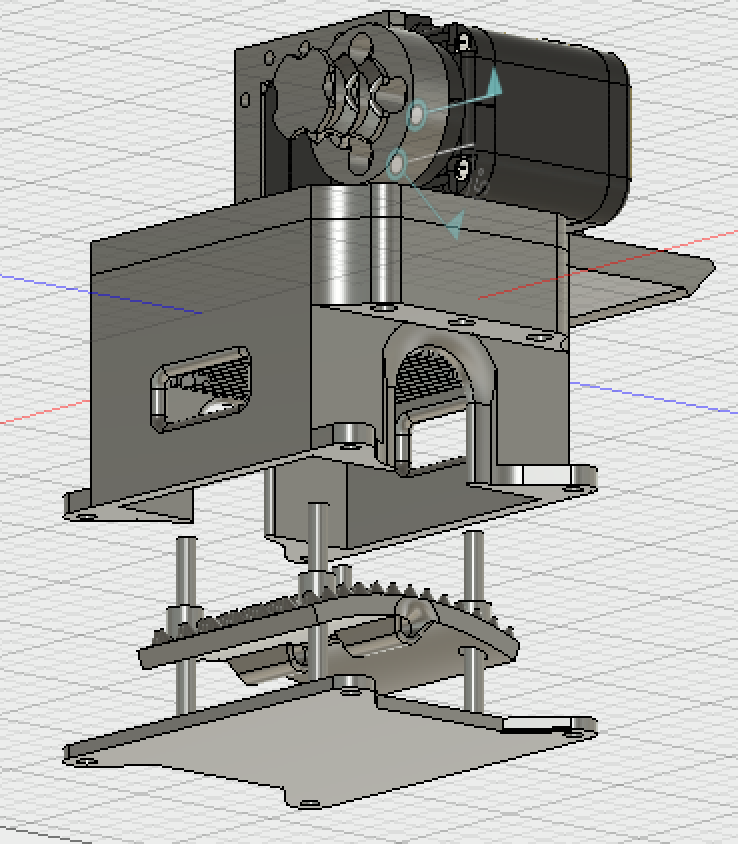
\includegraphics[scale=0.17]{exploded_gripper.png}
	\caption{Exploded view of clamp}
\end{figure}        
\subsubsection{Kinematic solution 1} \label{kinematic_solution_1}
To address the issues discussed in \ref{initial_kinematics}, the following kinematic model was produced. Since no rotational motions and no moment resistances are required at the end-effector, our kinematic model can be simplified to assume that all cables meet at a point ~\cite{WilliamsII2003} in the centre of our end-effector.
\begin{figure}
	\centering
	
	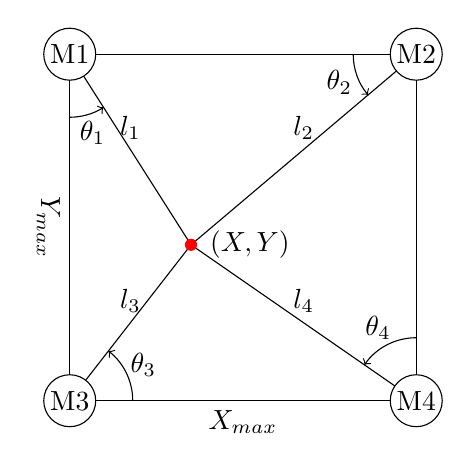
\begin{tikzpicture}[scale=1.1]
	
	\draw (0,0) -- (4,0) node[midway,below] {$X_{max}$} -- (4,4) -- (0,4) -- cycle node[midway,below,sloped] {$Y_{max}$}  ;
	
	\coordinate (M1) at (0,4);
	\coordinate (M2) at (4,4);
	\coordinate (M3) at (0,0);
	\coordinate (M4) at (4,0);
	\coordinate[label=right:{$\ (X,Y)$}] (c) at (1.4, 1.8);
	\draw (c) -- (0,0) node[midway,above] {$l_3$} ;
	\draw (c) -- (0,4) node[midway,above] {$l_1$} ;
	\draw (c) -- (4,0) node[midway,above] {$l_4$} ;
	\draw (c) -- (4,4) node[midway,above] {$l_2$} ;
	%\draw ()
	\fill[red] (c) circle (2pt);
	
	
	\draw[fill=white] (M3) circle (0.3cm) node[text=black] {M3};
	
	\draw[fill=white] (M1) circle (0.3cm) node[text=black] {M1};
	
	\draw[fill=white] (M4) circle (0.3cm) node[text=black] {M4};
	
	\draw[fill=white] (M2) circle (0.3cm) node[text=black] {M2};
	
	\pic [draw, angle radius=0.8cm, ->, "$\theta_1$", angle eccentricity=1.3] {angle = M3--M1--c};
	
	\pic [draw, angle radius=0.8cm, ->, "$\theta_2$", angle eccentricity=1.3] {angle = M1--M2--c};
	
	\pic [draw, angle radius=0.8cm, ->, "$\theta_4$", angle eccentricity=1.3] {angle = M2--M4--c};
	
	\pic [draw, angle radius=0.8cm, ->, "$\theta_3$", angle eccentricity=1.3] {angle = M4--M3--c};
	
	\end{tikzpicture}
	\caption{Kinematic diagram with point gripper} \label{fig:K_diag_1}
\end{figure}

Inverse Kinematics:
\begin{equation}
\cos(\theta_3) = \frac{X_{max}{}^2 + l_3{}^2 - l_4{}^2}{2*X_{max}*l_3}
\end{equation}
\begin{equation}
X = l_3\cos(\theta_3)
\end{equation}
\begin{equation}
Y = l_3\sin(\theta_3)
\end{equation}

Or, without trigonometry:

\begin{equation} \label{inverse_kinematics_1}
\begin{aligned}
&X = \left(\frac{X_{max}{}^2 + l_3{}^2 - l_4{}^2}{2*X_{max}*l_3}\right) = \frac{X_{max}}{2} + \frac{l_3{}^2 - l_4{}^2}{2*X_{max}}\\ \\
&Y = \left(\frac{Y_{max}{}^2 + l_4{}^2 - l_1{}^2}{2*Y_{max}*l_3}\right) = \frac{Y_{max}}{2} + \frac{l_4{}^2 - l_1{}^2}{2*Y_{max}}
\end{aligned}
\end{equation}

Forward Kinematics:
\begin{equation} \label{forward_kinematics_1}
\begin{aligned}
&l_1 = \sqrt{\left(X\right)^2 + \left(Y_{max}-Y\right)^2}\\
&l_2 = \sqrt{\left(X_{max}-X\right)^2 + \left(Y_{max}-Y\right)^2}\\
&l_3 = \sqrt{\left(X\right)^2 + \left(Y\right)^2}\\
&l_4 = \sqrt{\left(X_{max}-X\right)^2 + \left(Y\right)^2}\\
\end{aligned}
\end{equation}

\subsubsection{Control Software}
A Teensy 3.2 was configured to use the rosserial library to receive the targets CofM from the computer. The teensy then offset the coordinate system so that pixel 0,0 was in the centre of the image. The teensy kept track of all motor positions, and when a new CofM arrived the current gripper position was calculated from the motor positions using the forward kinematics. The x and y error between the centre of the camera image and the target is calculated, generating a vector that points towards the target, also known as visual servoing. This vector is translated into the change in length of each cord required to centre the gripper over the tracked target using the inverse kinematics \ref{inverse_kinematics_1} in \ref{kinematic_solution_1}. The desired gripper location is checked to see if it has left the bounds of the working area. If it has,motion along the axis which has been breached is set to zero. Finally, motor speeds are calculated from the desired changes in lengths as is described in \ref{motor_speed_equation} \ref{motor_speed_section}.

\subsection{Vision Algorithms}
An ideal object tracking algorithm would be algorithmically simple, quick to process, and be rugged against the various error sources vision systems encounter, whilst reliably detecting the location of the unknown object with some metric of how far away it is. Several algorithms were attempted to achieve this somewhat ambitious target. The four attempted algorithms will be briefly summarised below.

\subsubsection{Changing Histograms}
The first method was intended to provide a metric to identify interesting objects for further analysis. Histograms, using various colour channels, can be used to define how much of an image is dedicated to a given colour and light intensity. As an object approaches a camera it becomes larger, and thus consumed more of the image which should manifest as a positive rate of change over relevant histogram sections.

A significant issue prevented this algorithm from being used. Specifically, as an object travels, the lighting over the object changes and distributes itself inconsistently across the histogram. This is more prevalent indoors, and using a camera with fixed settings may have improved the situation.

\subsubsection{Optical Flow (Farneback)}
Optical flow can break up the motion between two frames of an image into lateral and vertical movements. As an object increases in size between images its motion can be used to create an outline around the object. This method was hampered due to interference from horizontal and vertical movements, where methods to reduce this became too complex to implement within the projects timeframe.

\subsubsection{Kalman filter}
To protect against the object being obscured when moving towards the gripper a 2D Kalman filter was implemented. It was found that, whilst an acceptable prediction of object position was calculated, the object was often lost before its maximum height was reached. This resulted in the prediction from the Kalman filter continuing vertically, making the solution inappropriate for our purpose. In future work as it is possible to estimate the velocity of a ball of known size from its circumference in the camera feed it is would be possible to combine this with our 2d Kalman filter to acquire a 3d estimate of trajectory. If an algorithm was produced to detect the ball had reached its maximum height and had begun falling, the predictive features of the Kalman filter could be used to help with latency issues and slow motors.

\subsubsection{Pyramid Scaling}
The third method revolved around how smaller objects would show up less on lower resolution images and is equivalent to using a variety of difference of Gaussians (DoGs) to detect edges and attempting to determine the size of an object between the DoGs. The main issue with this method was, again, lateral motion hiding the depth information.

\subsubsection{YOLO}
As a final method the You Only Look Once (YOLO) neural-network based object detection system was implemented to detect a small sample of objects. This method was hampered again by hardware capabilities as, even with YOLO-Tiny, a maximum of 7 frames per second were achieved which was considered too slow for the projects application.\subsection{Further problems}\subsubsection{Kinematics}\label{kinematic_solution_3}
Initially the kinematic solution considered the gripper as a point. This worked for preliminary testing, but soon proved to be a problem when the limited torque of the stepper motors required equal tension on all cords at all times. This led to the development of the following kinematic model, which considered the gripper as a square. 
\begin{figure}
	\centering
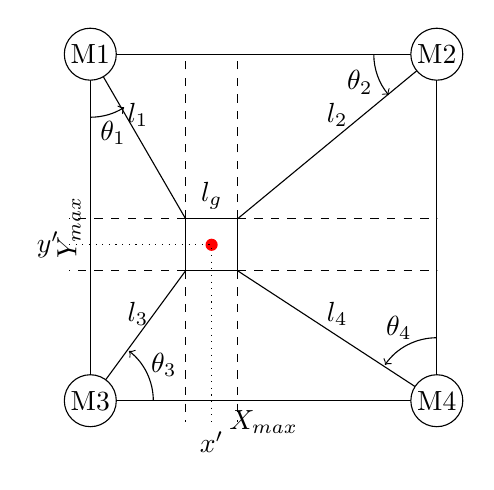
\begin{tikzpicture}[scale=1.1]

\def\gripSize{0.3}
%\pgfmathsetmacro{\grip_size}{0.3}

\coordinate (M1) at (0,4);
\coordinate (M2) at (4,4);
\coordinate (M3) at (0,0);
\coordinate (M4) at (4,0);

\draw (M3)--(M4) node[midway,below] (xaxis) {$X_{max}$};
\draw (M4)--(M2) node[midway,above](yaxisr){};
\draw (M1)--(M2) node[midway,right](xaxist){};
\draw (M3)--(M1) node[midway,above,sloped] (yaxis) {$Y_{max}$}  ;

%\draw (M3,M1) node (yaxis){};

\coordinate (c) at (1.4, 1.8);
\coordinate (c1) at ($(c) + (-\gripSize,\gripSize)$);
\coordinate (c2) at ($(c) + (\gripSize,\gripSize)$);
\coordinate (c3) at ($(c) + (-\gripSize,-\gripSize)$);
\coordinate (c4) at ($(c) + (\gripSize,-\gripSize)$);
\draw (c1) -- (0,4) node[midway,above] {$l_1$} ;
\draw (c2) -- (4,4) node[midway,above] {$l_2$} ;
\draw (c3) -- (0,0) node[midway,above] {$l_3$} ;
\draw (c4) -- (4,0) node[midway,above] {$l_4$} ;

%\draw ()
\fill[red] (c) circle (2pt);

\draw[dotted] (yaxis |- c) node[left] {$y'$}
-| (xaxis -| c) node[below] {$x'$};

\draw[dashed] (c3) -- (xaxis -| c3) ;
\draw[dashed] (c3) -- (yaxis |- c3) ;

\draw[dashed] (c1) -- (xaxist -| c1) ;
\draw[dashed] (c1) -- (yaxis |- c1) ;

\draw[dashed] (c2) -- (xaxist -| c2) ;
\draw[dashed] (c2) -- (yaxisr |- c2) ;
\draw[dashed] (c4) -- (xaxis -| c4) ;
\draw[dashed] (c4) -- (yaxisr |- c4) ;

\draw (c1) -- (c2) node[midway,above] {$l_g$} -- (c4) -- (c3) -- cycle;

\draw[fill=white] (M1) circle (0.3cm) node[text=black] {M1};

\draw[fill=white] (M2) circle (0.3cm) node[text=black] {M2};

\draw[fill=white] (M3) circle (0.3cm) node[text=black] {M3};

\draw[fill=white] (M4) circle (0.3cm) node[text=black] {M4};



\pic [draw, angle radius=0.8cm, ->, "$\theta_1$", angle eccentricity=1.3] {angle = M3--M1--c};

\pic [draw, angle radius=0.8cm, ->, "$\theta_2$", angle eccentricity=1.3] {angle = M1--M2--c};

\pic [draw, angle radius=0.8cm, ->, "$\theta_4$", angle eccentricity=1.3] {angle = M2--M4--c};

\pic [draw, angle radius=0.8cm, ->, "$\theta_3$", angle eccentricity=1.3] {angle = M4--M3--c};

\end{tikzpicture}
\caption{Kinematic diagram with square gripper}
\end{figure}
\linebreak

Inverse Kinematics:

\begin{equation}
\begin{aligned}
&X = \frac{X_{max}}{2} + \frac{l_3{}^2 - l_4{}^2}{2\left(X_{max} - l_g\right)}\\ \\
&Y = \frac{Y_{max}}{2} + \frac{l_3{}^2 - l_4{}^2}{2\left(Y_{max} - l_g\right)}\\
\end{aligned}
\end{equation}

Forward Kinematics:

\begin{equation}
\begin{aligned}
&l_1 = \sqrt{\left(X - \frac{l_g}{2}\right)^2 + \left(Y_{max}-Y+\frac{l_g}{2}\right)^2}\\
&l_2 = \sqrt{\left(X_{max}-X+\frac{l_g}{2}\right)^2 + \left(Y_{max}-Y+\frac{l_g}{2}\right)^2}\\
&l_3 = \sqrt{\left(X-\frac{l_g}{2}\right)^2 + \left(Y-\frac{l_g}{2}\right)^2}\\
&l_4 = \sqrt{\left(X_{max}-X+\frac{l_g}{2}\right)^2 + \left(Y-\frac{l_g}{2}\right)^2}\\
\end{aligned}
\end{equation}

\subsubsection{Skipping steps}\label{motor_issues}
The prototype was assembled with SST58D3820 stepper motors and TB6600 drivers. The TB6600 is designed to deliver up to 3.5A RMS. The drivers current can be limited down to 0.8A RMS in eight steps. Performance in the SST58D3820 datasheet is rated for when the motors are being supplied with 2.0A per phase. From this, we can see that the stepper motor requires 250mA per phase more than the driver can provide. When the robot was switched on the motors could barely hold the weight of the gripper when stationary. Experiment \ref{stepperReliability} was performed with the results showing that the stepper driver would not be suitable for this robot. This issue could have been partly mitigated if the motors were encoded.

\subsubsection{Motor velocities}\label{motor_vel_problem}
For the tension to remain equal on all cords during motion of the gripper, the motors must turn at different rates. For example: if the gripper starts in the centre of the frame and moves upwards, the top two lengths will shorten and the bottom two cords will get longer. To maintain a uniform velocity of the gripper, the top two motors must slow down and the bottom two must speed up. For gripper trajectories constrained to the centre of one axis this isn't much of a problem, but for trajectories traversing multiple axis the motors pull against each other resulting in steps being skipped and tension lost.






\section{Implementation}
\begin{figure}\label{fullPicture}
	\centering
	
	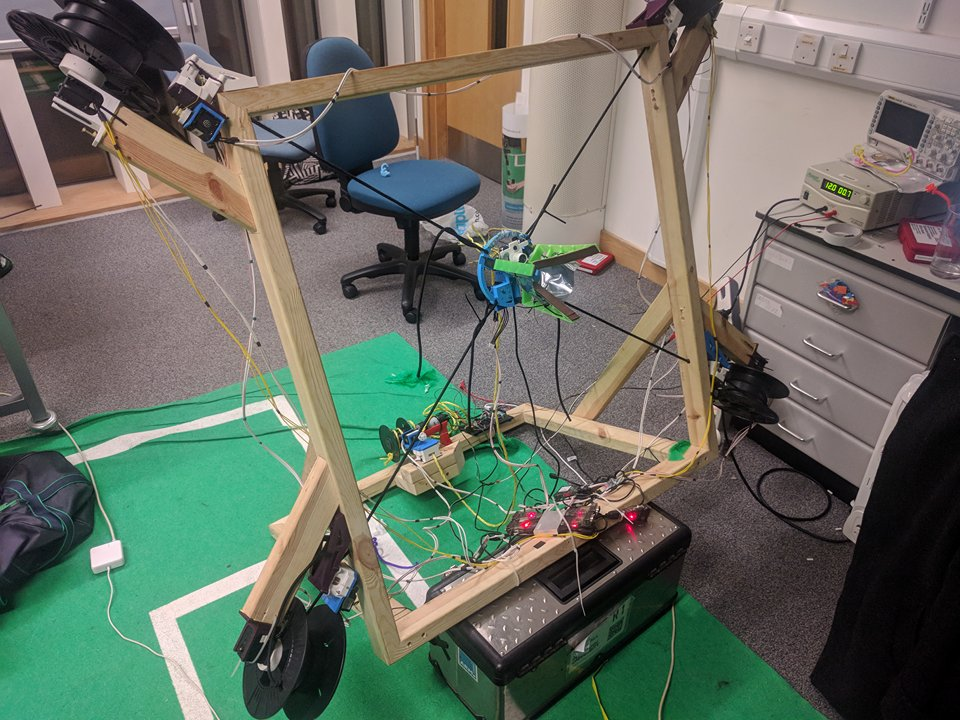
\includegraphics[scale=0.20]{finished_robot.jpg}
	\caption{The final prototype}
\end{figure}
\subsection{Software}
Frames enter the object tracking node at a rate of 60FPS. The object tracker performs a series of filters in different colour spaces on the image before calculating its centre of mass. This coordinate is published to the kinematic controller 17.5ms after the frame enters the object tracker. Upon entering the kinematic controller, the coordinate frame is offset so that the centre of the camera image is now at pixel 0,0. The required change in length of each cord is then calculated and set (via the method described in \ref{kinematic_solution_3}). From the desired changes in length, the required speed of each motor is calculated and set. The kinematic controller node then calculates the current gripper position in order to calculate the changes in length for the next loop.
Figure~\ref{fig:HighLevelDiagram} shows the high-level software flow diagram of the robot.



% Define block styles
\tikzstyle{decision} = [diamond, draw, fill=blue!20, 
text width=4.5em, text badly centered, node distance=3cm, inner sep=0pt]

\tikzstyle{block} = [rectangle, draw, 
text width=5em, text centered, rounded corners, minimum height=4em]

\tikzstyle{square} = [rectangle, draw, 
text width=5em, text centered, minimum height=4em, minimum width=7em]

\tikzstyle{sectionb} = [rectangle, draw, dotted, minimum height=18em, minimum width=12em, distance=0cm]

\tikzstyle{sectiona} = [rectangle, draw, dotted, minimum height=12em, minimum width=12em, distance=0cm]

\tikzstyle{label} = [rectangle, text width=5em]

\tikzstyle{line} = [draw, -latex']
\tikzstyle{cloud} = [draw, ellipse,fill=red!20, node distance=3cm,
minimum height=2em]
\begin{figure}[htbp]
	\centering
	\begin{tikzpicture}[node distance = 2cm,transform shape, scale=0.5]
	% Place nodes
	\node [square] (filter) {Filtering};
	\node [block, left of=filter, node distance=3cm] (camera) {Camera};
	\node [square, below of=filter] (CofM) {Centre of Mass};
	\node [square, below of=CofM, node distance=3cm] (lengthCal) {Calculate/set new lengths};
	\node [square, below of=lengthCal] (speedCal) {Calculate/set speeds};
	\node [block, left of=speedCal, node distance=3cm] (motors) {Motors};
	\node [square, below of=speedCal] (gripperPos) {Find gripper position};
	
	\node [sectionb, right of=speedCal, node distance =0.3cm] (section2) {};
	
	\node [right of=filter, node distance =0.3cm] (section1b4) {};
	
	
	\node [sectiona, below of=section1b4, node distance =1cm] (section1) {};
	
	\node [label, right of=section1, node distance =3.4cm] (labelA) {Object tracker};
	
	\node [label, right of=section2, node distance =3.4cm] (labelA) {Kinematic Controller};
	%    \node [label={[label distance=1cm]30:Object tracker}, right of=sectiona] {node};
	\node [right of = gripperPos] (dir1){};
	%    \node [join, above of = dir1] (dir2){};
	%    \node [above of = dir2] (dir3){};
	\node [right of = speedCal] (dir4){};
	% Draw edges
	\path [line] (camera) -- (filter);
	\path [line] (filter) -- (CofM);
	\path [line] (CofM) -- (lengthCal);
	
	\path [line] (lengthCal) -- (speedCal);
	\path [line] (speedCal) -- (gripperPos);
	\path [line] (lengthCal) -| (motors);
	\path [line] (speedCal) -- (motors);
	\path [line] (motors) |- (gripperPos);
	
	\path [line] (gripperPos) -| (dir4.center) |- (lengthCal);        
	
	\end{tikzpicture}
	\caption{High-level software flow diagram.}
	\label{fig:HighLevelDiagram}
\end{figure}

\subsection{Motor velocities}\label{motor_speed_section}
To address the issue raised in \ref{motor_vel_problem} a simple speed scaling system was devised. This algorithm was called once per main loop after the required changes in lengths are calculated. The algorithm takes in the requested changes in length of each cord and divides each change in length by the largest. The relative speeds of each motor are then scaled by the global speed scalar.
\begin{equation}\label{motor_speed_equation}
\begin{aligned}
&\vec{l} = \begin{bmatrix}
l_1\\l_2\\l_3\\l_4\\
\end{bmatrix}\quad
%&x = \max\{l_1,...,l_4\}\\
&x = \max\left(\vec{l}\right)\\\\
&x = \max\vec{l}\\\\
&\vec{s} = \frac{g}{x}\cdot \vec{l}\\
%&s_1 = \frac{l_1}{x}\\
%&s_2 = \frac{l_2}{x}\\
%&s_3 = \frac{l_3}{x}\\git sat
%&s_4 = \frac{l_4}{x}\\
\end{aligned}
\end{equation}
Where $g$ is the global speed scalar and $s$ contains the speed of each motor. 
\subsection{Servos and multi-threading}
Due to the points mentioned in \ref{motor_issues} the decision was made to change the motors to Dynamixel MX-64 servos. The MX-64 can supply $60Kg.cm$ at 62 RPM, giving a top gripper speed of $0.32m/s$ which is considerably slower than our requirement. The MX-64 servos communicate over either an RS-485 or a TTL bus and can be daisy-chained if required. Due to the nature of the communication protocols involved in the dynamixel bus (clarify), the rate at which commands could be sent to each servo were reduced with each successive servo added to the daisy chain. Initially the four servos responsible for translating the end-effector were daisy-chained to a single dynamixel bus resulting in a command rate of 7Hz. This was increased to 15Hz by increasing the baud rate of the servos from 57.6kb/s to 1Mb/s. The reduced control rate led to the decision to use separate busses for each time-critical motor resulting in a command rate per motor of 60Hz. Another bus was used for all five clamps, and a final sixth bus was used to actuate the gripper as the uncertainty of the command latency to this servo was required to be as low as possible in order to successfully pre-empt and act upon the target landing in the gripper. 

When a change in servo speed is requested, the dynamixel driver blocks the process thread that requested the change. The driver waits for a response from the motor before it allows the thread to continue. This reduced the rate at which motor instructions left the kinematic controller program to 10Hz. Creating four additional process threads for each of the speed-set service calls brought the loop rate back to 60Hz.

\subsection{Elastic cords}
Using bungee cord as the cable to drive the system has two benefits. Firstly, co-contraction can be used to alter the tension in the cable which allows the system. Either, to increase tension whilst moving (increasing the accuracy of the gripper), or to reduce tension when an object reaches the gripper. This allows the deceleration time of the object to be varied, resulting in less shock to the caught object and allowing more time for the gripper to close. Furthermore, the bungee can be used to store force which can be used to propel an object out of the gripper.

\subsection{Processor}
As servos were to be used instead of stepper motors, a microcontroller was no longer required for the control of the end-effector. Software previously running on the Teensy (forward/inverse kinematics, boundary checking etc...) was ported to a C++ program on a laptop running ROS on Ubuntu. 

\subsection{Throw Sequence}
Once a ball is caught, the internal state machine switches to throwing mode. The first step here is to either aim where to throw the ball or to centre the gripper to shoot forwards. This is then followed by tensioning the four outer motors, calibrating how far the ball should be thrown, and clamping their respective cables to store the energy.

The firing sequence consists of pulling the gripper, using the back motor, a set distance; clamping to store the added energy; unwinding the back motor so as to be able to be able to throw continuously without the use of manual resets, and unclamping the back motor to release the gripper forwards. A short time after releaseing, the gripper opens up to release the ball and, eventually, the four side motors are similarly unclamped, ready to catch another ball.

\subsection{Grippers}
Due to the complexities of gripper design, two distinct grippers were constructed.
\subsubsection{Soft Passive Gripper}
A soft passive gripper design was created due to the simplicity and speed of manufacture. Figure [figure 2] shows an image of the finished gripper.
Being 3D printed from PLA meant a prototype could be rapidly made and tested for functionality. With legs detachable from the gripper frame, several different designs and configurations could be tested. The legs went through multiple designs iterations, improved by finite element analysis (FEA) models. Stresses and deflections of the system were modelled using a static force of 1N applied uniformly over the catching face.

Several designs were tested, varying the number and thickness of the struts. ABS, rubber (as an analogue to NinjaFlex) and PLA (after importing the material properties ~\cite{CRF3:CRF3126}) materials were tested. Figure \ref{fea1}figure 3, 3mm] shows the FEA results for the finalised design.

\begin{figure}\label{fea1}
	\centering
	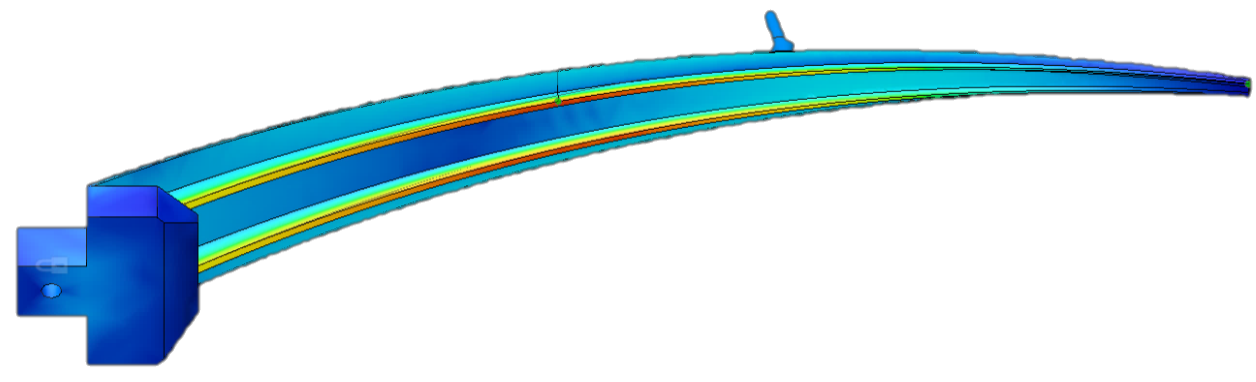
\includegraphics[scale=0.15]{fea1.png}
	\caption{Finite Element Analysis of one leg of the passive gripper}
\end{figure}

Due to the FEA iterative design process the legs worked as expected on the first print, with only minor design modifications to attach to the frame necessary. The object to be caught was initially a stress-ball which was used to generate requirements for the passive gripper. This was eventually replaced with a tennis ball, which meant the legs were sometimes too weak to capture it. 
\subsubsection{Soft Active Gripper}
The soft active gripper design has the potential to guarantee that objects (if caught) won’t slip out, and can more readily accommodate a larger variety of objects. Figure \ref{active_gripper} shows an image of the finished gripper.
\begin{figure}
\centering
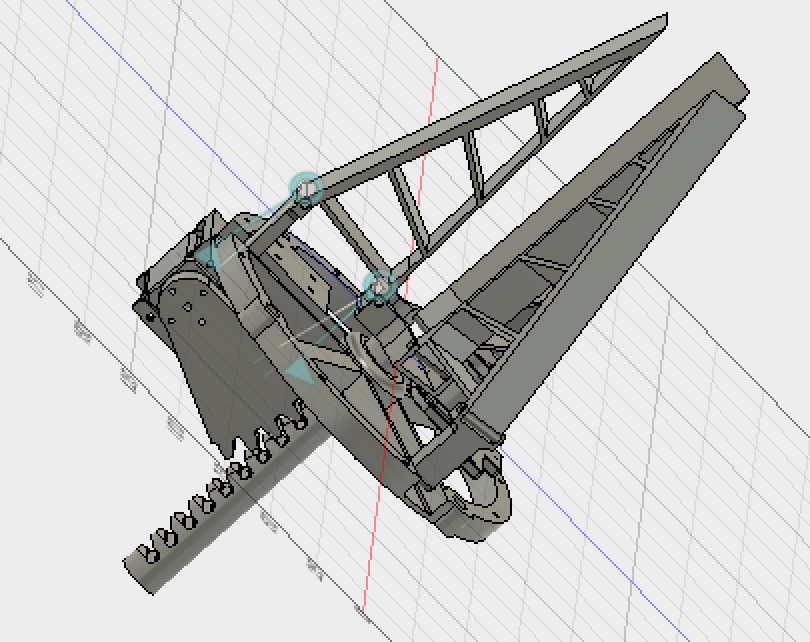
\includegraphics[scale=0.2]{active_gripper.png}
\end{figure}
The design, which is predominantly a replica of FESTO’s Fin Gripper~\cite{festofin}, was selected due to its tried and tested nature and overall simplicity. A CAD model of the design was edited to add a means of actuating the gripper, three methods were considered; first was a slider-crank mechanism, however, this was decided against due to the size of the mechanism that would be needed to actuate the gripper. Second, the gripper was redesigned to add a rack-pinion gear to each finger to enable actuation. This was decided against as this would have required three extra dynamixel motors with large gears to actuate each finger at an acceptable speed. The final design altered the shaft which actuates the gripper to be used as a rack gear which could then be actuated by a single dynamixel motor.




\subsection{Camera}\label{camera}
The finalised camera setup incorporated a single PS3-Eye camera in an eye-in-hand configuration. The PS3-Eye was selected due to several useful characteristics:
\begin{itemize}
	\item 187fps at 320x240 resolution
	
	\item Software-modifiable camera properties
	
	\item Lightweight after removing the casing
	
	\item \pounds0.50 at time of purchase
\end{itemize}

Owing to the high frame rate, motion blur became less of a concern when using the eye-in-hand configuration, which allowed for a simplified control algorithm. The camera can be seen attached to the active gripper in Figure [figure 4].

\subsection{Object Tracking}
The final object tracking algorithm could reliably track a red tennis ball up to 4 meters away. It was found that colour thresholding was the only solution to object tracking which could be developed within the time frame of the project, whilst also providing reliable, high-speed object recognition. An object is selected by clicking on the centre of the object in the camera feed. An average value for hue, saturate and variance (HSV) is then found from pixels surrounding the point selected. Using the HSV values, a minimum and maximum value are created by offsetting the average values by a predefined amount. These HSV values are then used to create a binary thresholded image which is dilated to remove image noise which appear as black speckles. Contour detection is performed on the binary image, the output contours are then run through OpenCVs minEnclosingRect function which will create the minimum rectangle which encloses the entire contour. To remove some unwanted contours, the difference of height and width of each created rectangle are compared and the contour is rejected if the difference is too large. With the remaining contours, a difference between the previously accepted objects CofM and the CofM of each contour is taken. The difference is used to find the distance between the previously accepted objects CofM and the contours CofM, the contour with the smallest distance is then accepted to be the object and published to the kinematic controller.

\section{Experiments}\label{experiments}
\subsection{Stepper Driver Performance}\label{stepperReliability}
\subsubsection{Method}
To assess the performance of the TB-6600, an experiment was performed where commands were sent to the robot instructing the gripper to move to the top corner and then return to the centre with cord lengths measured before and after. 
\subsubsection{Results}
It was found that requesting any movement of the gripper resulted in the stepper motors skipping steps, often resulting in the gripper dropping tens of centimetres over short movements. 
\subsubsection{Discussion}
Further investigation showed that the stepper drivers were drawing minimal current, and would overheat and shutdown if their current limit was set to more than half of what they were rated for. Even with a current limit set at 2.0A RMS, each stepper never drew more than 1.0A. This experiment showed that these drivers would not be suitable to drive the stepper motors in our project as they could not drive the stepper motors anywhere close to the specifications in the motors datasheet.


\subsection{Object tracking program rate}
\subsubsection{Method}
Timers were added to the object tracking program. The system time was taken when a camera frame entered the program and again when a CofM left the program. The difference in time was saved to a file every time the program looped. The program was run for ten minutes, after which a mean was calculated from the saved durations.
\subsubsection{Results}
The recorded loop rate of the object tracking program was $17.5ms$, or 57Hz.
\subsubsection{Discussion}
The camera frame rate during this test was set to 60Hz. As the recorded loop rate is close to 60Hz, it is believed that the object tracking module could complete a loop faster than the camera could generate frames. A useful future experiment would be to also calculate the duration between the object tracking module finishing and a new camera frame arriving.


\subsection{Kinematic controller rate}
\subsubsection{Method}
Timers were added to the kinematic controller program. The system time was taken when a coordinate entered the program and again when motor positions and speeds were published. The difference in time was saved to a file every time the program looped. The program was run for five minutes after which a mean was calculated from the saved durations.
\subsubsection{Results}
The kinematic controller takes $17ms$ to run, giving a loop rate of 60Hz.
\subsubsection{Discussion}
This experiment was performed in order to see whether latencies in the kinematic controller were preventing the robot from catching the ball. The program only runs when a CofM from the object tracking program arrives. As the camera frame rate was set to 60Hz during this experiment, it was concluded that the kinematic controller was probably completed before the next CofM arrived. A useful future experiment would be to also calculate the duration between the program finishing and a new CofM arriving. 

\subsection{Camera latency}
\subsubsection{Method}
The camera was connected to a computer and the video feed was viewed on the computer monitor. The camera was pointed at a digital stopwatch on a smartphone so that the stopwatch could be seen on the computer monitor. A second camera was orientated so that both the stopwatch and the computer monitor showing the video of the stopwatch could be seen and a photograph was taken. 
\subsubsection{Results}
The photograph on the second camera showed a time of 4.187 seconds on the computer monitor and 4.112 seconds on the stopwatch. The difference in these times is $75ms$ which is the latency of the USB camera used to track the ball in this project.

\subsubsection{Discussion}A thrown ball travelling at $5m/s$ at 45\degree\ will be falling at approximately $3.5m/s$ when it falls past the height at which it was thrown.  A latency of $75ms$ results in the ball falling $26cm$ further than the camera reports. Without predictive algorithms, this latency will prevent the system from working correctly.


\subsection{Catching Performance}
\subsubsection{Method}
A ball was thrown twenty times from three meters away from the final version of the robot with the thrower aiming at the gripper, and 20 times with the thrower aiming within the frame but not at the gripper. The robot was angled so that the gripper was raised by 25\degree\ towards the ceiling. 
\subsubsection{Results}
The robot caught the ball seven out of twenty times when the ball was aimed at the gripper. When the ball was not aimed at the gripper, the robot did not catch the ball once.
\subsubsection{Discussion}
The robot does not perform as originally designed. The main issue is the speed of the servos and the camera latency.


\section{Overall Discussion}\label{overall}
\subsection{Overall Discussion}
From the experiments performed it is clear that the object tracking and gripper-object coordination challenges were successfully solved throughout this project. It is also clear that, even with a functioning system, there is still much work left to be done. This section shall briefly review each of the 6 challenges, outlining successes and areas of further development.

\subsection{Body Design}
Although the system does function, experiment E clearly shows that it is non-functional. There is no single root cause, however, experiment A indicates that motor selection and power is, and has been, a continuous issue throughout this project. As such, a clear design improvement would be an improved motor and motor driver setup.
Also noted in the methodology of experiment E is how the robot is tilted during the experiment. This was because it was observed to have an improved reliability at this angle. Hence, another improvement and test set would involve a built-in mechanism to alter the robots inclination and determine usability at various levels.

\subsection{Gripper Design}
Although an experiment was not explicitly created to test the gripper functionality, it was observed that both passive and active grippers functioned reliably as intended. The passive gripper had an issue with the ball passing straight through it when thrown at a high enough velocity, so a recommended improvement would be incorporating netting toward the back to prevent this.
Further developments in gripper design would involve creating and testing hard versus soft gripper designs.

\subsection{Camera Setup}
The camera setup worked with reasonable success. Given the high fps and resolution of the camera, objects were reliably trackable even in the eye-in-hand configuration. However, Experiment D provides insight into the main failure of this setup, camera latency. This is a difficult issue to resolve with standard USB 2.0 based cameras. A recommended improvement would be sourcing a camera using the USB 3.0 protocol or investing in other communication systems to resolve this issue.

\subsection{Object Tracking}
Experiment B indicates that the tracking algorithm requires little processing to go from a raw input to a tracked object. However, this setup is limited to balls of known colour, preferably red. This is a huge limitation on the systems capabilities. As such, further development would involve trialling various different tracking algorithms to allow a wider range of objects to be detected. Testing under more lighting conditions and environments, to ruggedise against related errors, would also help improve the system.

\subsection{Gripper-Object Coordination}
Via the use of encoded motors in the MX-64's, and a reliable tracking algorithm, the system control was successful. Experiment A demonstrates the necessity for the motor encoders, however, other alternatives could be devised to alleviate this requirement and enable a wider range of motors to be selected for improved body design. One such method would be to use distance sensors on the gripper to determine its x-y coordinate.

\subsection{Object Grasping}
The scope of this project did not allow for complex gripper designs, so advanced object manipulation has not been accomplished. Having said this, although the throwing mechanism is untested, it does function. Improvements to this setup would involve accurate mathematical models to determine the distance and trajectory of a thrown object, as well as determining a control algorithm to throw in the desired direction.

\section{Conclusion}
This document has outlined the development process for a CDDR catching and throwing robot. The resulting system used under-specified components due to the originally sourced motors underperforming and budget constraints. A reliable control system with positional and object location feedback was presented. Two successful gripper designs were created for the purpose and were functionally analysed.

Further development would involve sourcing motors capable of achieving the desired tasks, and modifying the base so as to more readily experiment with angled catchment areas. Detailed models of the stored energy in the throwback mechanism, along with expected trajectory planning, would also be of use.

% conference papers do not normally have an appendix


% use section* for acknowledgment
\section*{Acknowledgment}


The authors would like to thank Dr Martin Stoelen for his support, resourcefulness and guidance throughout the duration of this project.


	
	
	% trigger a \newpage just before the given reference
	% number - used to balance the columns on the last page
	% adjust value as needed - may need to be readjusted if
	% the document is modified later
	%\IEEEtriggeratref{8}
	% The "triggered" command can be changed if desired:
	%\IEEEtriggercmd{\enlargethispage{-5in}}
	
	% references section
	
	% can use a liography generated by BibTeX as a .bbl file
	% BibTeX documentation can be easily obtained at:
	% http://mirror.ctan.org/biblio/bibtex/contrib/doc/
	% The IEEEtran BibTeX style support page is at:
	% http://www.michaelshell.org/tex/ieeetran/bibtex/
	\bibliographystyle{IEEEtran}
	% argument is your BibTeX string definitions and bibliography database(s)
	%\bibliography{IEEEabrv,../bib/paper}
	%
	% <OR> manually copy in the resultant .bbl file
	% set second argument of \begin to the number of references
	% (used to reserve space for the reference number labels box)
	\bibliography{ROCO504}{}
	\bibliographystyle{IEEEtran}
	

	
	
	% that's all folks
\end{document}


